\documentclass[11pt]{article}
\usepackage{color}
\usepackage{natbib}
\usepackage{graphicx}
\setlength{\oddsidemargin}{0in}
\setlength{\textwidth}{6.5in}
\setlength{\textheight}{9.2in}
\setlength{\topmargin}{-.40in}
\setlength{\headheight}{0in}
\setlength{\footskip}{1.5cm}
\usepackage{times}
\setlength{\parindent}{35pt}
\begin{document}

\begin{center}
 {\large   \sf Reply to reviewer's and associate Editor}\\
    \vspace{.1in}
    March 12, 2018
  \end{center}
\section{Reply to associate editor}
{\color{blue}{Associate Editor (Remarks to Author):\\

Both reviewers commented on the switch to a dry-mass vertical coordinate but with opposite reactions. I think it would be helpful to the paper, and to assuage \# 1, by providing more evidence of the benefits of the switch to dry-mass. Other than that, I think the paper fits the purpose of a documentation paper for the CESM special issue.}}

The author's thank the associate editor for supporting the publication of this manuscript after the appropriate revisions are made. In the response to reviewer 1 we will address the associate editors overall comment. Also, we have performed a slight rewording of the title from `NCAR CESM2.0 release of CAM-SE: ...' to `NCAR release of CAM-SE in CESM2.0'.
\section{Reply to reviewer 1}
We thank the reviewer for the helpful comments and spending the time going through a long and technical manuscript. Responses are interleaved below (reviewer comments are in blue font and authors responses in black font). 
\subsection{Reviever 1's overall comments}
{\color{blue}{
This is a well-written and mostly comprehensive paper describing a new dynamical core, and should be published to document the advances described within and the dynamical core characteristics.}}

{\color{blue}{
 I do feel that some of the major changes compared with the earlier CAM-HOMME are not well-justified, while some of the improvements demonstrated (especially with regard to the kinetic energy spectrum) are a re-configuration of the model and not intrinsic to the core formulation.}}\\

Agreed! The reduction of the viscosity coefficients and changes to the vertical remapping could also have been applied to CAM-HOMME and has little to do with the reformulation in dry-mass vertical coordinates. In the results section we show that for the experiments we perform the main differences between CAM-HOMME and CAM-SE are due to viscosity changes, vertical remapping changes and treatment of the energy conversion term in the thermodynamic equation (Figure 7) that could also have been applied to CAM-HOMME.\\

We would like to elaborate further on the viscosity changes: It is correct that the improvement in the TKE is due to the rescaling of the hyperviscosity coefficients. That said, there have been important changes to how the viscosity is applied that has allowed for reduced damping. Simply reducing viscosity coefficient in CAM-HOMME would have led to an unstable simulation (especially with `real-world' topography). Applying the damping on approximate pressure levels rather than $\eta$-levels as well as only damping the deviations of damping pressure level thicknesses from reference thicknesses has allowed for the reduction in viscosity coefficients.\\

Changes to the manuscript: 
\begin{itemize}
\item In the abstract we have added `Not related to the vertical coordinate change, the hyperviscosity operators and the vertical remapping has been modified and ...' to alert the reader that not only has the vertical coordinate changed but also other aspect of the algorithm (not related to the vertical coordinate). has undergone further development.
\item Section 4.2 we have replaced the sentence `The increased kinetic energy at smaller scales is primarily the result reducing the explicit diffusion coefficients used in CAM-SE (not shown).' with `The increased kinetic energy at smaller scales is due to reducing the explicit diffusion coefficients used in CAM-SE compared to CAM-HOMME rather than the reformulation of the dynamical core in dry-mass vertical coordinates or a more comprehensive treatment of moist energy. Reducing the viscosity coefficients without increasing noise in the solutions (especially in the presence of `real-world' topography) has been made possible by damping momentum and temperature on approximate pressure levels and only damping the deviation of pressure-level thickness from a smoother reference pressure-level thickness.'
\item In the Introduction, paragraph 2, we have added the following sentence: `The basic spectral-element method has not been changed but we present changes to the details of how hyperviscosity is applied and the vertical remapping that are not specific to the dry-mass vertical coordinate.' 
\item We have modified wording (red font) in the conclusions: `In particular, we show that the reduction in viscosity parameters {\color{red}{(made possible by changes to the details of how hyperviscosity is applied)}} greatly improved the total kinetic energy spectrum of CAM-SE and that the comprehensive treatment of moist thermodynamics and condensate loading significantly changes precipitation rates in aqua-planet simulations. {\color{red}{These changes are not due to the dry-mass vertical coordinate per se but we argue that the comprehensive treatment of energy in the Earth system model as a whole is much simpler in a dry-mass vertical coordinate (for example, a dry-mass vertical coordinate does not change during parameterization updates).}}'


%In the conclusions we have added the sentence: `These changes are not due to the dry-mass vertical coordinate per se but we argue that the comprehensive treatment of energy in the Earth system model as a whole is much simpler in a dry-mass vertical coordinate which stays fixed during parameterization updates.'
\end{itemize}

{\color{blue}{
While interesting from a design standpoint, I am not convinced that the change from moist-mass to a dry-mass vertical coordinate represents an improvement to the model, despite the great effort that would be required for this change, inside and outside of the core. The main justification given is that it makes a number of parts of the model ``easier'', although it is not clear that this is the case. While it may eliminate the need to rescale tracer masses, now the mass effect of water vapor and the condensates needs to be explicitly added in when computing the pressure-gradient force, among other considerations. It is also mentioned in Section 4.2 that many parts of the physics would need to be re-written to work with dry mass; most notably, the use of dry mass leads to the inequality of the hydrostatic assumption in (47), which is a very common assumption in models (presumably more common than the assumption that pressure surfaces do not change). }}\\

We agree that within the dynamical core the change to a dry mass vertical coordinate makes the code more complicated in terms of having to add up all water tracers to get the full pressure and similarly in the hydrostatic equation. The argument for moving to dry mass vertical coordinates  is to move towards an Earth system model with a more accurate treatment of energy and we argue that is simpler to do in a dry-mass vertical coordinate (considering all aspects of the model - not just the dynamical core). We decided to make this change in the dynamical core first before attempting to formulate physics in a dry-mass vertical coordinate. As the reviewer mentions, this will require significant changes on the physics side - but it will also be an opportunity to get a more consistent treatment of total energy in the parameterizations (e.g., take into account work done by water leaving the column). All of this could, in theory, be done in a moist coordinate but at the expense of less clear separation of the terms in the energy equation.\\ 

Another motivation (not mentioned in the manuscript) for the dry-mass vertical coordinate is the consistent coupling between CAM-SE and CSLAM \cite[Conservative Semi-LAgrangian Multi-tracer scheme][]{LNU2010JCP} in a moist atmosphere. The consistent coupling between the SE continuity equation for air and the continuity equation for tracers (solved with CSLAM) is much more consistent in a dry-mass coordinate as explained in the following. In a dry-mass formulation CSLAM transports water tracers while SE solves the continuity equation for dry air. The two are consistently coupled by making sure that if a tracer has value 1 (in which case CSLAM predicts the evolution of dry air mass) then the CSLAM dry mass field is identical to the SE dry mass field integrated over CSLAM control volumes \citep[how this is done is explained in detail in ][]{LTOUNGK2017MWR}. Had one used a moist vertical coordinate then this coupling between SE and CSLAM would be complicated by the fact that water tracers would implicitly be predicted by SE through solving the continuity equation for moist air mass (using a moist vertical coordinate).\\


Changes to manuscript:\\

\begin{itemize}
\item In the introduction we made the following change:\\

Including the thermodynamic and mass effect of condensates in the dynamical core using a dry-mass hybrid-sigma vertical coordinate {\color{red}{is mathematically simpler due to the clear separation of dry air, water vapor and condensates in the discretization.}} This is the initial motivation for using a dry-mass vertical coordinate. {\color{red}{That said, certain parts of the implementation of a dry-mass coordinate in the dynamical core is slightly more complicated since moist pressure is a diagnostic in a dry-mass vertical coordinate formulation  (mass effects of moisture and condensates need to be explicitly added)} whereas in a moist coordinate pressure is prognostic.}
\item The following paragraph has been added to the introduction:\\

`The fourth motivation for a dry-mass formulation is the consistent coupling between CAM-SE and CSLAM \cite[Conservative Semi-LAgrangian Multi-tracer scheme][]{LNU2010JCP} in a moist atmosphere. The consistent coupling between the SE continuity equation for air and the continuity equation for tracers (solved with CSLAM) is much more consistent in a dry-mass coordinate as explained in the following. In a dry-mass formulation CSLAM transports water tracers while SE solves the continuity equation for dry air. The two are consistently coupled by making sure that if a tracer has value 1 (in which case CSLAM predicts the evolution of dry air mass) then the CSLAM dry mass field is identical to the SE dry mass field integrated over CSLAM control volumes \citep[how this is done is explained in detail in ][]{LTOUNGK2017MWR}. Had one used a moist vertical coordinate then this coupling between SE and CSLAM would be complicated by the fact that water tracers would implicitly be predicted by SE through solving the continuity equation for moist air mass (using a moist vertical coordinate). Hence a dry-mass formulation benefits CAM-SE-CSLAM version of CAM-SE that share the same code base.'
\end{itemize}

{\color{blue}{
Other than the moist-mass effects, have there been any fundamental improvements to the discretization in CAM-SE? Some of the changes demonstrated in the paper are just re-configuration of runtime parameters. Figure 6 shows a major change in the kinetic energy spectrum, but this should be simply due to the new choice of parameters, and doesn't seem to be due to fundamental improvements in the solver. }}\\

In addition to the  changes in the equations of motion (comprehensive and energetically consistent treatment of all forms of water), there have been significant changes in the way hyperviscosity is applied (i.e. applied to approximate pressure-levels rather than $\eta$, and different pressure-level thickness damping) as well as vertical remapping changes (mapping thermal energy instead of temperature and turning off limiters for momentum mapping). The basic spectral-element solver remains the same.\\

Changes to the manuscript: In the Introduction, paragraph 2, we have added the following sentence: `The basic spectral-element method has not been changed but we present changes to the details of how hyperviscosity is applied and the vertical remapping that are not specific to the dry-mass vertical coordinate.' 

\subsection{Reviever 1's minor comments}
\begin{itemize}
\item {\color{blue}{ Section 2: I would dispute the claim that the ``governing equations for moist atmosphere flows remain...active research'', as the appropriate thermodynamics of moist air is well-understood (Emanuel 1994 is a good reference). What is true that it is unclear how to best represent moist dynamical effects in numerical models. This has been discussed at length in several papers, including Ooyama (1990, 2001) and in Satoh (2003).


Emanuel, K., 1994: Atmospheric Convection. Oxford University Press, 580 pp.\\

Ooyama, K. V., 1990: A thermodynamic foundation for modeling the moist atmosphere. J. Atmos. Sci., 47, 2580-2593.\\

--, 2001: A dynamic and thermodynamic foundation for modeling the moist atmosphere with parameterized microphysics. J. Atmos. Sci., 58, 2073-2102.\\

Satoh, Masaki. ``Conservative scheme for a compressible nonhydrostatic model with moist processes.'' Monthly weather review 131.6 (2003): 1033-1050.}}

Agreed!\\

Change to the manuscript: Sentence replaced with `While the appropriate thermodynamics of moist air is well-understood \citep[e.g.][]{E1994} it is unclear how to best represent moist dynamical effects in numerical models \citep{O1990JAS,O2001MWR,S2003MWR,B2003JAS}.'

\item {\color{blue}{Section 2.5: Is there a justification for using T as the prognostic variable instead of potential temperature, which is conserved in adiabatic flows? This is important because the calculation of omega can be quite delicate (Holton 2004, 3.5.1), and must be accurately computed to ensure energy conservation in this equation.}}

This is mostly done for historical reasons.  CAM has long relied on a
discrete hydrostatic integral consistent with a prognostic temperature
and conventional pressure gradient \cite{CAM5}. The
discrete system conserves energy to time truncation error even with
moisture \cite{T2011LNCSEb}.  We are currently 
evaluating a potential temperature formulation which requires the
pressure gradient to be written in terms of Exner pressure and a
different discretization of the hydrostatic integral, requiring
additional modifications to the CAM physics routines.\\

That said, the potential temperature and Exner pressure formulation is ill-conditioned for high-top applications (above the homopause) and CAM-SE is currently being implemented into WACCM and WACCM-x (which are high top models).



\item {\color{blue}{Also in section 2.6: You make reference to the ``specific damping coefficients''. Shouldn't these be runtime-parameters? I presume that the best value of the damping will depend on the application (for example, data assimilation cycling may benefit from additional damping to remove short-wavelength waves due to imbalances) and may not be a simple function of resolution.}}

The authors agree. The `specific' coefficients where determined emperically for stability and may have to be increased for specific applications. The sentence\\

`The specific damping coefficients for divergence ($\nu_{div}$), vorticity ($\nu_{vor}$), level-thickness ($\nu_p$) and temperature $(\nu_T)$ are resolution specific and provided in Appendix A.3.'\\

has been replaced with \\

`The damping coefficients for divergence ($\nu_{div}$), vorticity ($\nu_{vor}$), level-thickness ($\nu_p$) and temperature $(\nu_T)$ are resolution dependent and provided in Appendix A.3. These coefficients were determined empirically for stability and may have to be increased for specific applications such as data-assimilation cycling where additional damping to remove short-wavelengths due to imbalances may be necessary.'

\item {\color{blue}{ Section 3.3: I am unfamiliar with the spectral element method. In traditional finite-differencing schemes there is a well defined way for each grid point to be influenced by its neighbors. How does each element communicate with one another? Is it by the shared points on the edges of each element? Also, if indeed it is only by the edge points, then wouldn't a broader domain of dependence (with more points) be needed for a higher-order method?}}

Good question. The spectral element is `spectral' on each element so if, for example, one of the quadrature values is changed then it affects the basis functions throughout the element (but not the nodal values). The element `communicates' with other elements through the DSS operation where values on the element edges (where GLL nodes are shared) are averaged - that is how information is propagating between elements.\\

Changes to the manuscript: The following text has been added to the end of Section 3.3\\

'Note that nodes on the element boundary are shared between elements and that after each Runge-Kutta step the shared nodes will have different values. The elements are coupled by averaging the two solutions at the shared nodes (so the halo communicated between elements is only one node/point deep). This is referred to as the DSS operation. The solution is therefore only $C^0$ at element boundaries. The ability to obtain high-order accuracy with only edge point communication is an attractive feature of the spectral element method \cite{MadayPatera87,canuto2007}. Another aspect of the spectral element is that the basis function representation is spectral on each element so if, for example, one of the quadrature values are changed then it affects the basis functions throughout the element (except at the GLL nodes).'

\item {\color{blue}{Section 3.4: It is claimed that the SE method is energy- and mass- conserving. However the damping applied to the mass and temperature fields is said to not be energy conservative. How can you claim the method is energy conserving? Indeed, we see later (section 4.2.1) that even the adiabatic core is not energy conserving the way that mass-conservative schemes are able to conserve mass down to computational rounding error. Further, is the damping applied to the mass field mass-conserving? }}

That is indeed confusing language used in section 3.4. For the frictionless equations of motion (i.e. no hyperviscosity terms) the SE discretization is energy conserving to time-truncation errors. The hyper-viscosity on momentum is converted into heating so kinetic energy dissipation through hyperviscosity has a closed energy budget. Energy conservation is violated by hyperviscosity on temperature and pressure (a detailed energy analysis of CAM-SE is the subject of a manuscript currently in preparation). The damping applied to mass is mass-conserving to computational rounding error.\\

Changes to manuscript: section 3.4 has been reworded (changes in red font):\\

`This property can be used to show the inherent conservation properties of CAM-SE {\color{red}{in the horizontal discretization \citep[see ][ for details]{T2011LNCSEb}. Mass is conserved and, in the absence of viscosity terms, energy is conserved with exact timestepping}}. 

Since the CAM-SE discretization is mimetic the adiabatic, frictionless discretization of the equations of motion conserves total moist energy to within time-truncation errors. The equivalent internal energy change due to hyperviscosity damping of the velocity vector is added as frictional heating in the thermodynamic equation so the energy budget for the viscosity on the momentum equations is closed. The dissipation of energy due to hyperviscosity on temperature and dry-mass, however, is not energy-conserving. The vertical remapping does not conserve total energy either but it does conserve moist internal energy and AAM. {\color{red}{Hyperviscosity reduces variance but is a mass-conserving operation in CAM-SE.}}'

\item {\color{blue}{Section 4.2: Can you check to be sure that greater divergence damping does decrease the (resolved) vertical motion in your simulations? One might expect that much of the vertical motion will be parameterized in either case. Furthermore it is not necessarily true that increasing the divergence damping will lead to weaker precipitation systems:\\ 


Zhao, Ming, Isaac M. Held, and Shian-Jiann Lin. ``Some counterintuitive dependencies of tropical cyclone frequency on parameters in a GCM.'' Journal of the Atmospheric Sciences 69, no. 7 (2012): 2272-2283.}}

Thank you for this insightful comment. It is both interesting and consciously coincidental that we chose to use the word 'intuitive' here. We have looked into both the mean (Figure~\ref{fig:denergy}) and extreme values of omega, and find that the magnitudes decrease for the larger divergence damping coefficient, overall (for this configuration). The response is intuitive. An additional figure has been added to section 4.2 making this point clear. Some counter-intuitive responses may certainly occur in a different configuration/resolution, especially one permitting the formation of tropical cyclones. A line has been inserted in section 4.2 pointing to \cite{ZHL2012JAS}, acknowledging that the response to divergence damping coefficient is not always intuitive.

\begin{figure}[h]
\centering
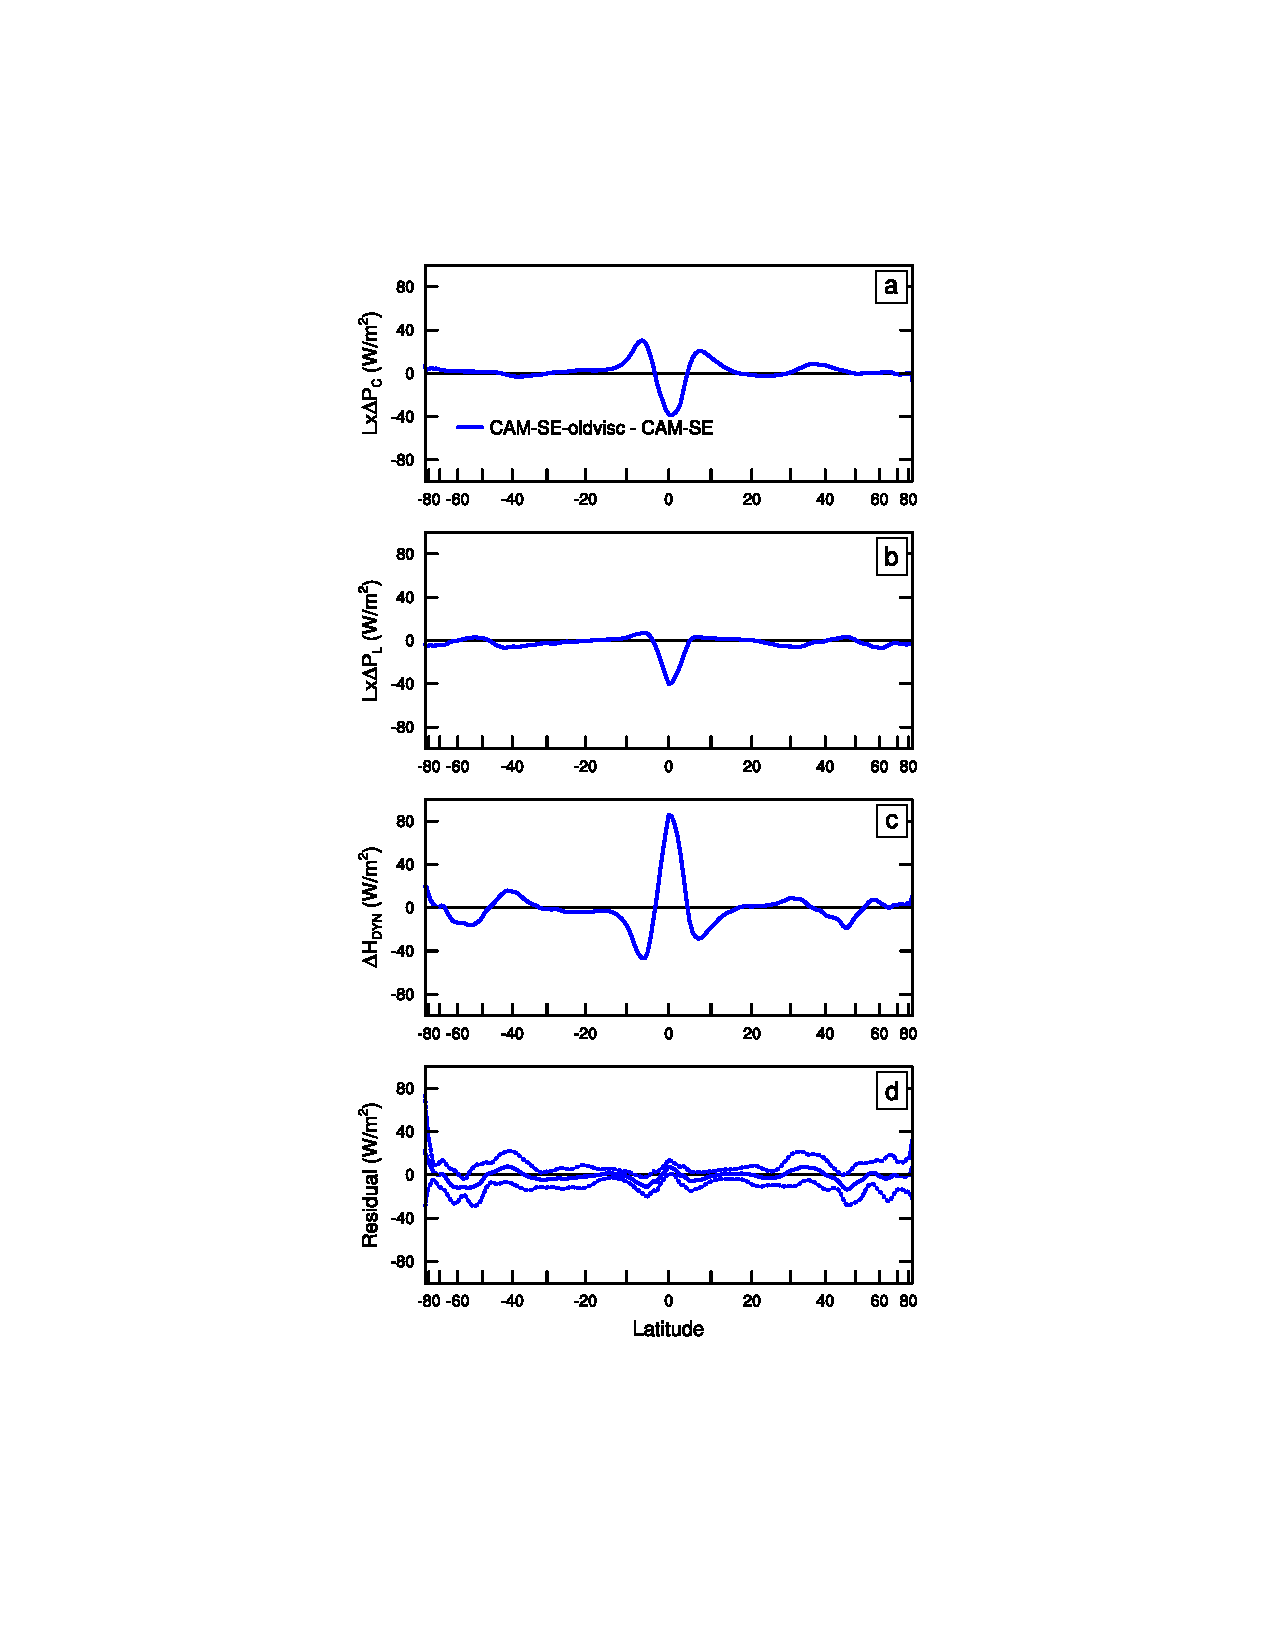
\includegraphics[width=20pc]{temp_denergy_SE_v_SE-oldvisc.pdf}
\caption{Departure of the components of the zonally averaged dry static energy budget between CAM-SE-lovisc and CAM-SE. Anomalous latent heat associated with (a) convective precipitation and (b) large-scale precipitation (c), the dynamical component of the anomolous divergence of the flux of dry static energy by the mean vertical circulion, and (d) the residual component from the sum of (a), (b) and (c). Dotted lines refer to twice the standard deviation associated with low frequency (monthly) variablity. The term in (c) is proportional to the change in omega, and is indicates anomolous heating owing to a reduction in the divergence of the mean vertical advective flux of dry static energy.}
\label{fig:denergy}
\end{figure}

\item {\color{blue}{Section 4.2.1: Again, we see that the dynamical core does not actually conserve angular momentum, but instead that it merely has a spurious imbalance smaller than that of the physics. }}

Correct!

\item {\color{blue}{Figure 6: It is difficult to get a sense of the physical scales in the kinetic energy spectrum plot. Could either a second axis showing physical wavelengths, or a line indicating 6dx or 4dx scales, be added to the plot?}}

6dx and 4dx lines, along with a separate axis with the implied wavelength, has been added to the figure.

\item {\color{blue}{Figure 7: Some of the colours, especially blue and purple, and red and magenta, are hard to tell apart. }}

We have changed the colors so as to be more readable.

\item {\color{blue}{Section 4.3: The performance gains in CAM-SE over CAM-HOMME are excellent. Is this due to code optimization, or have there been science-related changes that could also lead to speedups? Also, tracer advection can be a major cost in many numerical models. How many tracers are used for these benchmark tests, and how efficient is the tracer advection compared to the rest of the dynamics?}}

The performance gains in CAM-SE over CAM-HOMME are almost entirely due to improvements in code optimization. The new dry-mass formulation should actually be slower then the previous formulation if no code optimizations had been undertaken (moist pressure is diagnostic implying the summation of water every dynamics time-step for computing the pressure gradient force and hydrostatic integral, hyperviscosity is more complicated due to having to compute a reference pressure  - that requires communication - and the correction terms for approximate pressure-level damping).  The number of advected tracers is 33 in this case.  The vast majority of the performance gains were a direct result of improving the cache behavior in the advection algorithm.  \\

Changes to the manuscript:
\begin{itemize}
\item we have added that CAM6 has 33 advected species in the performance section.
\item added to sentence (red font):\\

`We suspect that the decrease in computational cost illustrated in Figure 11 is likely due to the fact that the calculations performed in the dynamical core {\color{red}{(in particular tracer advection code)}} now fit into the Level 3 (L3) cache on 75 nodes where they did not previously in either the original code base on the optimized code base on smaller node counts.  The decreased execution time due to the calculations being L3 cache resident is sufficiently large as to overcome any increase in execution time increase due to message passing.'
\end{itemize}

\item {\color{blue}{Appendix B: we see that the continuous equations are indeed mass, angular momentum, and energy conserving. How might the discretization affect these conservation relations? In particular, I had thought that the vector-invariant momentum equation (49) is not angular-momentum conserving; and the angular momentum conservation law (B.3) does not make the shallow-atmosphere approxmiation used in the rest of the text.}}

Angular momentum is not inherently conserved in discretizations based on the vector-invariant momentum equations; neither is the case for the kinematic momentum formulation used in, e.g., MPAS. In fact, it is unclear why some numerical methods conserve AAM better than others \citep[see ][]{LBDL2014JAMES} but we are unaware of discratizations inherently conserving AAM.\\

In (B.3) $r$ is the mean radius of Earth so the equation does make the shallow atmosphere approximation.\\

Changes to the manuscript: `CAM-SE uses the vector-invariant form of the momentum equations and the discretization thereof is not inherently AAM conserving' added to conclusions section.
\end{itemize}  
\newpage

\section{Reply to reviewer 2}
We thank the reviewer for the helpful comments and spending the time going through a long and technical manuscript. Responses are interleaved below (reviewer comments are in blue font and authors responses in black font). 
\subsection{Reviewer 2's overall comments}
{\color{blue}{This manuscript presents a documentation of the new NCAR CESM2.0 release of CAM-SE with its reformulated dynamical core that uses a dry-mass vertical coordinate and accounts for the condensate loading effects. The authors present in detail the continuous equations and their discretization, and present a few results from simplified experiments to demonstrate the effect of the reformulations and the conservation properties expected from the discretized equations of the dynamical core. A substantial appendix adds further details to the documentation. Overall I think that the paper fulfills its purpose, as it provides the necessary background information for the analysis of experiments based on this model or for its further development. The text is relatively hard to read, owing to the large number of necessary equations, but they are unavoidable.
In general I congratulate the authors for their decision to reformulate the dynamics with dry-mass vertical coordinate and with comprehensive treatment of condensates and energy. In reading the manuscript it one realizes only relatively late that this reformulation is still limited to the dycore. Therefore I would recommend to clarify early in the text that this paper presents the reformulation of the model dynamics (i.e. of the dynamical core) alone, while a reformulation of the physical parameterizations, as necessary for a fully consistent model, is a separate endeavor that will be addressed later (if that is the plan). Then less explanations about the lack of consistency are needed in the discussion of the results.
Otherwise I do not have any major critique. But please check carefully the equations. A number of minor errors are pointed out below.
I recommend a minor revision.}}

We agree that it is not entirely clear that this is a manuscript focusing on the dynamical core in the introduction. We do, however, advocate to keep the discussion of the lack of consistency with physics since we argue that is an important topic and relevant to this manuscript.

Changes to the manuscript:\\

In last paragraph of the introduction we have added the sentence: `This paper presents the reformulation of the SE dynamical core alone, while a reformulation of the physical parameterizations, as necessary for a fully consistent model in dry-mass vertical coordinates, is a separate endeavor.'
\subsection{Reviever 2's minor comments}
\begin{itemize}
\item {\color{blue}{L40: ``... the SE methods' near perfect scalability ...'' or ``... the near perfect scalability of the SE methods ...''}}

Fixed.

\item {\color{blue}{L46: explain ``equi-angular gnomonic'' or provide reference with explanation, maybe section 3 of Lauritzen et al. 2010 (doi:10.1016/j.jcp.2009.10.036) would do.}}

Added reference to \cite{RP1996QJ}. FYI: Regular gnomonic, equ-angular gnomonic and hybrid approach are compared in \cite{NTL2005MWR}.

\item {\color{blue}{L61: ``science changes'' is vague. Based on the title of the manuscript you could use ``... reformulations of the dynamical core ...''}}
 
Reformulated!

\item {\color{blue}{Figure 1: Panel (a) shows the spectral element grid for Ne=20, while panel (b) seems to use Ne=30 as a base grid. Also both panels show different rotations of the globe and (b) does not show the cubed sphere panel edges. Making the two panels as similar as possible would be helpful.}}

Done! Plots (a) and (b) are now centered over the US. (a) now shows $N_e=30$ grid and (b) shows the elements of the actual Conus grid (instead of a low resolution version).

\item {\color{blue}{L.80-102: From these two paragraphs, both motivating the utility of the dry-mass vertical coordinate, it somehow becomes clear that also the physical parameterizations are involved. But it is not sufficiently clear that for a fully consistent formulation of this CAM-SE and physics, also the physical parameterizations need (in part) to be reformulated so that the same definitions of cp and energy are in use through the whole model. Please add a statement that clarifies already here that (a) an adaptation of the physics is necessary for a fully consistent model, and that (b) this adaptation is not treated in this paper, but will follow later.}}

Good point. \\

Changes to the manuscript: The following sentence has been appended:\\

The changes to physics needed to make it consistent with the dynamical core (discussed in this paragraph and the previous paragraph) is necessary for a fully consistent model. This adaptation is, however, not treated in this paper.

\item {\color{blue}{L129: The first sentence is a bit awkward to read. Why not ``Equation 1 defines ... `` L159: ``... (more on this ...) ``}}

`Define the dry mixing ratios ...' changes to `Equation (1) defines the dry mixing ratios ...'\\

`(more on this ...)' changes to (see Section 2.4.2 ...)'

\item {\color{blue}{Eq. 22 and 23: For completeness one could add that (23) also uses $\partial S^{(l)}/\partial E^{(l)} = 1/T$}}

Added.

\item {\color{blue}{ Eq.26: ...$\alpha^{(l)} - V(cond)/V$  ...}}

Added. {\color{blue}{Is (26) correct.}}

\item {\color{blue}{L175: ... where $\alpha^{(l)} = V/N^{(l)}M^{(l)}$ is the ...}}

Corrected.

\item {\color{blue}{Eq.28 and 29: ... $d [(1-\xi^{(cond)})\alpha^{(l)}]$. }}

Corrected.

\item {\color{blue}{L177: ... i.e. $\xi^{(cond)} = 0.$}}

Corrected.

\item {\color{blue}{Eq.33-35: left hand side, 2nd term has wrong sign }}

Corrected.

\item {\color{blue}{Eq.33: ... - $\sum m^{(l)}\alpha^{(l)} p^{(l)}$ = ...}}

Sign corrected (previous bullet point) but the term is, to our knowledge, correct $\sum_{\ell \in \mathcal{L}_{gas}}m^{(\ell)} \alpha^{(\ell)}dp^{(\ell)}$.

\item {\color{blue}{Eq.34: ... -$1/\\rho^{(d)}\sum dp^{(l)} = $...}}

Corrected.

\item {\color{blue}{Eq.35: ... -$1/\rho dp = $...}}

Corrected.

\item {\color{blue}{L182: ... then using (13) the ...}}

Done

\item {\color{blue}{L195: ... We assume that the composition of dry air is constant and that there is no moisture ...}}

Done

\item {\color{blue}{Eq. 41, 42, 44: The integral of dz is in the increasing direction of z, so that dz is positive. With $\rho$ and $g$ being positive, and for a positive pressure, the signs should be changed:}}

Done

\item {\color{blue}{Eq.41: $p(z) = g$  ...}}

Done

\item {\color{blue}{Eq.42: $=g$...}}

Done

\item {\color{blue}{Eg.44: $M^{(l)}(z)$ = $< Integral>$}}

Done

\item {\color{blue}{L213-219: As physical explanation one could add that when hydrometeors are falling at terminal velocity, the gravitational force pulling the hydrometeors downward is compensating by the upward frictional force of the gaseous atmosphere on the hydrometeors. This compensating force adds to the atmospheric pressure.}}

Added to manuscript.

\item {\color{blue}{Eq.46: M is mass, not weight: $dM^{(d)}(z) = -\rho^{(d)} dz,$}}

Corrected

\item {\color{blue}{L225: ... only if there are no condensates present at higher levels ...}}

Added to manuscript.

\item {\color{blue}{L261: Numbering of appendices: currently the subsections of appendix A are numbered as A.1, A.2 and A.3. This numbering is also used for equations in Appendix A. Please use a different numbering of the appendix sections, e.g. A.a, A.b and A.c.}}

It is author's understanding that this change is up to the journal.

\item {\color{blue}{Please add a reference to Appendix A.1. I couldn't find any.}}

Appendix A.1 is referenced implicitly through the reference to Appendix A.

\item {\color{blue}{L261-264: Please add here the consequences of formally allowing different values for the viscosities $\nu_p, \nu_T, \nu_{div}$ and $\nu_{vor}$. I think it is important to know that the mass-wind consistency requires $\nu_p =\nu_{div}$, which is now ``hidden'' in the appendix A.3. What would be the consequence of $\nu_T \neq \nu_{vor}$?}}

Tracer / tracer-mass consistency requires $\nu_p = \nu_q$ (there was a typo in the manuscript; $\nu_p =\nu_{div}$), that is, the hyper-viscosity applied to density has to be the same as the hyper-viscosity applied to tracers.\\

There are no constraints on the hyper-viscosity coefficients applied to velocity, $\nu_{div}$ and $\nu_{vor}$.  Also, no constraints of the hyper-viscosity applied to temperature.\\

We have emperically found it effective to use a larger $\nu_{div}$ and $\nu_p$ compared to $\nu_T$ and $\nu_{vor}$ to damp computational modes and noise associated with the SE basis functions being $C^0$ at element boundaries.\\

We have not investigated what the consequence of  $\nu_T \neq \nu_{vor}$ is but it is, indeed, an interesting research question.\\

Changes to the manuscript: appended 'Note that the viscosity coefficient for pressure and tracers should be the same otherwise the model is no longer 'free-stream' preserving (i.e. a constant mixing ratio is preserved; also referred to as mass-wind consistency in the literature). The dispersion properties of CAM-SE with hyperviscosity are similar to A-grid models. There are no computational modes, but the grid scale modes are erratic with large phase errors \citep{AW2009SIAM}. Empirically we have found that increasing $\nu_{div}$ and $\nu_p$ compared to  $\nu_T$ and $\nu_{vor}$ is effective at damping grid-scale modes and noise associated with the SE basis functions being $C^0$ at element edges while not making the total kinetic energy spectrum too dissipative at the high wavenumbers.' after line 264.

\item {\color{blue}{Further it would be interesting to get insight in the factors between the viscosities. Why is it that CAM- SE needs ($\nu_p$, $\nu_{div}$) = 5($\nu_T$, $\nu_{vor}$)? Does CAM-SE have numerical modes in divergence? If you have some insight, it would be great to share it with the reader.}}

See answer to previous bullet point.

\item {\color{blue}{L279 and Eq.59: without factor 1/2.}}

Missing 1/2 added to equation 59.

\item {\color{blue}{L290-293: Also convection parameterizations matter, as a forcing for resolved waves, and the dissipation (numerical and physical) matters for the QBO.}}

Sentence at L290 has been replaced with:\\

`Good AAM conservation may be important for the simulation of the Quasi-Biennial Oscillation (QBO) although the accurate simulation of the QBO also depends on vertical resolution, location of model top, model dissipation (numerical and physical) and parameterizations \citep[such as nonorographic gravity wave drag and convection parameterization; ][]{RSB2014JGR}. '

\item {\color{blue}{L323-324: The sentence ``In the model code this is controlled ... `` is not really clear. What exactly is meant by ``this'' and what is meant be ``.true.''?}}

Clarified by replacing sentence with:\\

`CAM-SE's total energy can be made consistent with CAM physics (described above) and it is enabled/disabled in the model code with the  logical parameter $\tt{lcp\_moist}$.'

\item {\color{blue}{L.333: ``... and similarly for full levels k. ... ``: Please specify how $A_k$ and $B_k$ are defined for full levels.}}\\

Appended 'where $A_k=\frac{1}{2}\left( A_{k+1/2}+A_{k-/12}\right)$ and $B_k=\frac{1}{2}\left( B_{k+1/2}+B_{k-/12}\right)$'\\

\item {\color{blue}{L.342: ``... and density ...'': Later Eq.73 shows that density is defined on the full levels, not on the interface levels as stated on this line. What is correct?}}

Density is a derived variable and defined at full levels. Manuscript text corrected by removing density from L342.

\item {\color{blue}{Section ``3.5 Temporal discretization'':
This section details the rational for using different time stepping schemes for different equations or operations. What is missing is to point out if there exist any links between the schemes. In particular I am wondering how tracer mass conservation and mass-wind consistency is achieved with different schemes for advection and the continuity equation. Does the ``faster'' dynamics provide dry-air mass flux information from its se\_rsplit dynamics steps to the ``slower'' tracer advection step?}}

The choice of a 5 stage high-CFL RK method for dynamics and a 3 stage RK-SSP method
allows both dynamics and tracers to use the same timestep.  
For mass / tracer-mass consistency, the dynamics computes a mean flux (averaged over
the 5 Runge-Kutte stages.  This mean flux is then used by all 3 tracer RK stages.\\

Changes to the manuscript: The following sentence has been added to section 3.5, `The choice of a five stage large-timestep Runga-Kutta method for dynamics and a three stage RK-SSP method allows both dynamics and tracers to use the same timestep. For mass / tracer-mass consistency, the dynamics computes a mean dry-air mass flux (averaged over the five Runge-Kutte stages. This mean flux is then used by all three tracer RK stages.'

\item {\color{blue}{L545-550: Tracer concentrations need to be positive definite as outlined, which may require some sort of limiters. When water tracers are involved, such mechanisms, however, not only affect the tracer budgets, but generally also the energetics. Does CAM-SE relate tracer tendency limitations to the energetics? Or does ``setting to zero'' of a mixing ratio necessarily cause an energetic inconsistency? It would be valuable to have some explanation on this aspect.}}

Very interesting question. In the physics-dynamics coupling layer (that the reviewer is referring to) there is an if-statement to prevent tracer mass from becoming negative. That operation will be a spurious source if mass and energy for the forcing term. After submitting this manuscript the E3SM model (the DOE version of CESM using SE) group has showed that using the ftype=0 option leads to significant errors in coupled simulations due to the `clipping' of water sink terms \citep{water-leak}. Given this new information we will change ftype to 2 in CAM-SE in future applications of the model.\\

Changes to the manuscript: Appended the following sentence\\

`This leads to energy conservation errors and it has recently been shown to lead to hydrological cycle biases in coupled climate simulations \citep{water-leak}.'

%First of all, in the dynamical core where there are no phase changes, the latent heat contained in the tracers is proportional to their mass, and thus does not change (as long as we conserve mass).  And since the limiter in the transport scheme conserves mass (and dissipates variance) the global energetics should not change. Locally, of course, a limiter will change the local energy budget.\\



\item {\color{blue}{L586: ... Appendix D. When ...}}

The LaTeX style from JAMES adds `:' after the reference to the Appendix. Asking journal to fix.

\item {\color{blue}{L701: Please specify the model top of the 32 level version used here.}}

Top is at approxmately 3.6Pa. Added to text.

\item {\color{blue}{L706: ``... reducing the explicit diffusion coefficients used in CAM-SE'': Are all viscosity coefficients reduced equally? Or does the benefit origin from a more selective reduction ($\nu_{div}$ or $\nu_{vor}$)?}}

See answer to comment to L261-264.

\item {\color{blue}{L803-806: If the explanations outlined in Fig.8 holds, the same effects should unfold in realistic experiments, though they might be less visible.}}

Agreed.

\item {\color{blue}{L830-835: What is the expectation for the physical torque? Is the observed wind torque consistent with AAM variations of the atmosphere, or does Fig.9 show some inconsistency in the physics?}}

The torque from physics is not total AAM conserving so Figure 9 is not showing inconsistency from physics. The purpose of comparing the physics torque to the dynamical core torque is to show that the spurious torque from dynamics is much less than the `physical' torque from physics.

Sentence in L830 changed to (changes in red font):\\

As discussed in Section 2.7 the total AAM torque from the dynamical core, in the absence of topography, should be small {\color{red}{(ideally zero)}} compared to the torque from the parameterizations {\color{red}{which is not spurious}}.

\item {\color{blue}{L873: ... cores/node. The x-axis ...}}\\

Fixed.

\item {\color{blue}{L905-907: Fig. 11 shows that the fraction of the dycore costs is reduced for higher node numbers, as a result of the ``super-scaling'' illustrated in Fig. 10. Then other fractions must increase as the total relative costs = 1 is constant. Therefore from Fig.11 - without more information - we cannot learn if physics costs have remained constant (=''perfect scaling'') or possibly changed. The same holds for the other parts. My suggestion is to replace Fig.11 by a new figure that shows the costs of each part (I/O, dynamics, physics \# dynamics, physics) similar as in Figure 10, with costs scaled by the costs of the 5-node setup of the CAM-SE. Additionally a line for the costs of the ``whole model'' should be shown for completeness.}}\\

We have modified figure 11 (which is Figure 12 in the new version of the manuscript) such that it illustrates the core-hours per simulated year for each sub-component of CAM as well as the entire atmosphere model. After the submission of our initial manuscript we identified an errant print statement that was causing scalability issues in the physics section of the code. The affect of this print statement was significant at larger core counts, and now the physics illustrates only a very minor increase in cost at greater then 30 nodes.\\

Figure 14 has also been updated.

\item {\color{blue}{L1315: probably ... (2014) ...}}

Fixed.

\item {\color{blue}{Figure 7: The colors for CAM-SE and CAM-SE-ppmlimiter are difficult to distinguish. Please find better colors.}}

We have changed the colors as to be more readable.

\item {\color{blue}{Figure 8a: Use bigger font!}}

The font size has been increased.

\item {\color{blue}{Figure 11: There is only one panel \# ``(a)'' not needed, and the text for panel (b), which obviously has become Figure 12, must be deleted.}}

Fixed.

\end{itemize}
\bibliographystyle{abbrv}
\bibliography{bib}
\end{document}

